
% Slideshow, written by Brent Baccala, for a lecture at TJHSST

\documentclass{beamer}
\usetheme{Madrid}

\title{A New Solution to Hydrogen}
\author{Brent Baccala}
\institute{\tt cosine@freesoft.org}
%% \date{February 8, 2023}

\setbeamertemplate{footline}{}
\beamertemplatenavigationsymbolsempty

\usepackage{amsmath}
\usepackage{tabularx}

\usepackage{breqn}

\usepackage{xcolor}
\usepackage{comment}
\usepackage{graphicx}

\usepackage{tabularx}

\usepackage{tikz}
\usetikzlibrary{positioning}
\usetikzlibrary{fit}
\usetikzlibrary{backgrounds}

\usepackage{adjustbox}

\def\coeff{\framebox(10,10){}}
\newcommand{\tikzmark}[1]{\tikz[overlay,remember picture] \node (#1) {};}

\begin{document}


\begin{frame}
\titlepage
\begin{block}{Abstract}
A New Solution to Hydrogen
\end{block}
\end{frame}

\begin{frame}
\begin{exampleblock}{}
\begin{center}
\vskip 20pt
\Huge
Part 1: Schr\"odinger's Equation
\vskip 6pt
\ 
\end{center}
\end{exampleblock}
\end{frame}

\begin{frame}
\frametitle{Force, Field, Potential, Potential Energy}
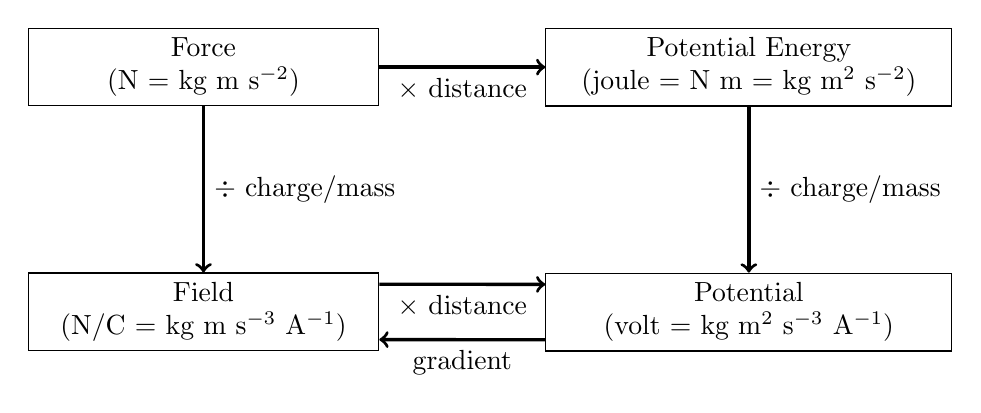
\begin{tikzpicture}[node distance=60pt]
\node (force) [draw, text width=120pt, align=center] {Force\\(N = kg m s$^{-2}$)};

\node (field) [below=of force.south, draw, text width=120pt, align=center] {Field\\(N/C = kg m s$^{-3}$ A$^{-1}$)};

\node (energy) [right=of force.east, draw, text width=140pt, align=center] {Potential Energy\\(joule = N m = kg m$^2$ s$^{-2}$)};

\node (potential) [below=of energy.south, draw, text width=140pt, align=center] {Potential\\(volt = kg m$^2$ s$^{-3}$ A$^{-1}$)};

\draw [very thick, ->] (force.south) -- (field.north) node[pos=0.5,right] {$\div$ charge/mass};
\draw [very thick, ->] (energy.south) -- (potential.north) node[pos=0.5,right] {$\div$ charge/mass};
\draw [very thick, ->] (force.east) -- (energy.west) node [pos=0.5, below] {$\times$ distance};
\draw [very thick, ->] ([yshift=10]field.east) -- ([yshift=10]potential.west) node [pos=0.5, below] {$\times$ distance};
\draw [very thick, <-] ([yshift=-10]field.east) -- ([yshift=-10]potential.west) node [pos=0.5, below] {gradient};

\end{tikzpicture}
\end{frame}

\begin{frame}
\frametitle{Hamiltonian Mechanics}
\end{frame}

\begin{frame}
\frametitle{Probability Density Functions}
\end{frame}

\def\argt{(\vec{x}_1,...,\vec{x}_n,t)}
\def\arg{(\vec{x}_1,...,\vec{x}_n)}

\begin{frame}
\frametitle{The Wave Function}
\[ \Psi\argt \]

The {\bf wave function} is a complex-valued function of position and time that encodes
probability density functions for both the position and momentum of all particles.
It is a function of the coordinates of {\it all} particles.

\begin{quotation}
Example: The wavefunction of a two particle system:

\[ \Psi(x_1,y_1,z_1,x_2,y_2,z_2,t) \]
\end{quotation}

The square amplitude of the wave function gives the probability density of the position.

The square amplitude of its Fourier transform gives the probability density of the momentum.

\[ \Phi(p) = \frac{1}{\sqrt{2\pi\hbar}}\int \Psi(x)e^{-\frac{i}{\hbar}px}dx \]
\end{frame}

\begin{frame}
\frametitle{(Time Dependent) Schr\"odinger Equation}
%% \includegraphics[clip, trim=0in 5.6in 0in 0.75in, width=\textwidth, page=1]{GrobnerBasis.pdf}
%% \includegraphics[clip, trim=0in 6.25in 0in 0.5in, width=\textwidth, page=9]{GrobnerBasis.pdf}
%% \includegraphics[clip, trim=0in 3in 0in 0.5in, width=\textwidth, page=13]{GrobnerBasis.pdf}
\[ \hat{H} \Psi\argt = i \frac{\delta}{\delta t} \Psi\argt \]
%\vskip 0.3in
\begin{center}
\underline{{\bf Definition of Hamiltonian operator $\hat{H}$}}
\[ \hat{H} \Psi\argt = \hat{T} \Psi\argt + \hat{V} \Psi\argt \]

$\hat{T}$ is the kinetic energy operator

$\hat{V}$ is the potential energy operator

\[\hat{T} = \sum_i - \frac{\hbar^2}{2m_i}\nabla_i^2 \qquad\qquad \hat{V} = V\argt\]

\[ \nabla_i^2 = \frac{\delta^2}{\delta x_i^2} + \frac{\delta^2}{\delta y_i^2} + \frac{\delta^2}{\delta z_i^2} \quad {\rm (cartesian\ coordinates)}\]

the sum in $\hat{T}$ is over all particles

\end{center}

\end{frame}

\begin{frame}
\frametitle{Time Independent Schr\"odinger Equation}
If the potential energy $V\argt$ has no time dependence, we can 
use separation of variables and {\it assume} that the wavefunction has the form:

\[ \Psi\argt = \psi\arg\phi(t) \]

\[\sum_i - \frac{\hbar^2}{2m_i}\nabla_i^2 \psi\arg\phi(t) + V\arg\psi\arg\phi(t) \]
\[ = i \frac{\delta}{\delta t} \psi\arg\phi(t) \]

divide through by $\psi\arg\phi(t)$:

\[ \frac{1}{\psi\arg} \left[ \sum_i - \frac{\hbar^2}{2m_i}\nabla_i^2 \psi\arg + V\arg\psi\arg \right] \]
\[ = \frac{i}{\phi(t)} \frac{\delta}{\delta t} \phi(t) \]

\[ \hat{H} \Psi = E \Psi \]
\end{frame}

\begin{frame}
\frametitle{Time Independent Schr\"odinger Equation}
If the potential energy $V\argt$ has no time dependence, we can 
use separation of variables and {\it assume} that the wavefunction has the form:

\[ \Psi\argt = \psi\arg\phi(t) \]

\[\sum_i - \frac{\hbar^2}{2m_i}\nabla_i^2 \psi\arg\phi(t) + V\arg\psi\arg\phi(t) \]
\[ = i \frac{\delta}{\delta t} \psi\arg\phi(t) \]

divide through by $\psi\arg\phi(t)$:

\[ \frac{1}{\psi\arg} \left[ \sum_i - \frac{\hbar^2}{2m_i}\nabla_i^2 \psi\arg + V\arg\psi\arg \right] \]
\[ = \frac{i}{\phi(t)} \frac{\delta}{\delta t} \phi(t) \]

\end{frame}

\begin{frame}
\frametitle{Time Independent Schr\"odinger Equation}
The time part:

\[ E = \frac{i}{\phi(t)} \frac{\delta}{\delta t} \phi(t) \qquad\Rightarrow\qquad - i E \delta t = \frac{\delta\phi(t)}{\phi(t)} \qquad\Rightarrow\qquad - i E t + C = \ln \phi(t) \]
\[ \phi(t) = e^C e^{-iEt}\]

The position part:

\[ \frac{1}{\psi\arg} \left[ \sum_i - \frac{\hbar^2}{2m_i}\nabla_i^2 \psi\arg + V\arg\psi\arg \right] = E \]

\[ \left[ \sum_i - \frac{\hbar^2}{2m_i}\nabla_i^2 \psi\arg + V\arg\psi\arg \right] = E \psi\arg \]

The combined time independent Schr\"odinger equation:

\[ \hat{H} \psi\arg = E \psi\arg \qquad\qquad \Psi\argt = e^{-iEt} \psi\arg\]
\end{frame}

\begin{frame}
\frametitle{Hartree Atomic Units}
{\bf Hartree Atomic Units} is a system of units in which four fundamental physical constants
are assigned the value of 1:
\begin{itemize}
\item the reduced Planck constant ($\hbar$)
\item the elementary charge ($e$)
\item the electron rest mass ($m_e$)
\item the Coulumb constant ($k_e$)
\end{itemize}

The unit of distance (Bohr radii) is approximately half an angstrom.\\
\qquad \AA = $10^{-10}$ m (NaCl inter-atomic distance is about 2.8 \AA)

The unit of time is 24 as (1 attosecond = $10^{-18}$ s).

The speed of light is approximately 137.

The unit of energy is the Hartree, approximately 27.2 eV.
\end{frame}

\begin{frame}
\frametitle{Simple Atomic or Molecular Schr\"odinger Equation}

In atomic units, the Hamiltonian for $N$ electrons and $M$ nuclei is:

\[ \hat{H} = - \sum_{i=1}^N \frac{1}{2} \nabla_i^2 - \sum_{A=1}^M \frac{1}{2M_A}\nabla_A^2 - \sum_{i=1}^{N}\sum_{A=1}^M \frac{Z_A}{r_{iA}}
+ \sum_{i=1}^{N}\sum_{j>i}^N \frac{1}{r_{ij}} + \sum_{A=1}^{M}\sum_{B>A}^M \frac{Z_A Z_B}{R_{AB}}
 \]

%% In the above equation:
\begin{itemize}
\item $ \nabla_i^2 = \frac{\delta^2}{\delta x_i^2} + \frac{\delta^2}{\delta y_i^2} + \frac{\delta^2}{\delta z_i^2}$ (cartesian coordinates)
\item $M_A$ is the ratio of the mass of the nucleus $A$ to the mass of an electron
\item $Z_A$ is the atomic number of nucleus $A$
\item only electrostatic forces; no magnetic forces, no electrodynamics
\item no relativistic effects
\end{itemize}

\vfill
Source: Szabo and Ostlund, {\it Modern Quantum Chemistry}, eq (2.2), p.41
\end{frame}

\begin{frame}
\frametitle{Hydrogen Schr\"odinger Equation}

\[ \psi(x,y,z) \]

\[ r = \sqrt{x^2+y^2+z^2} \]

\[ \hat{H} = \frac{1}{2} \nabla^2 - \frac{1}{r}  \]

\[ \frac{1}{2} \nabla^2 \psi(x,y,z) - \frac{1}{r} \psi(x,y,z) = E \psi(x,y,z) \]

\[ \frac{1}{2} \frac{\delta^2 \psi(x,y,z)}{\delta x^2} + \frac{1}{2} \frac{\delta^2 \psi(x,y,z)}{\delta y^2} + \frac{1}{2} \frac{\delta^2 \psi(x,y,z)}{\delta z^2} - \frac{1}{r} \psi(x,y,z) = E \psi(x,y,z) \]

\end{frame}

\begin{frame}
\frametitle{Helium Schr\"odinger Equation}

\[ \psi(x_1,y_1,z_1,x_2,y_2,z_2) \]

\[ r_1 = \sqrt{x_1^2+y_1^2+z_1^2}   \qquad\qquad r_2 = \sqrt{x_2^2+y_2^2+z_2^2} \]
\[ r_{12} = \sqrt{(x_2-x_1)^2+(y_2-y_1)^2+(z_2-z_1)^2} \]

\[ \hat{H} = \frac{1}{2} \nabla_1^2 + \frac{1}{2} \nabla_2^2 - \frac{1}{r_1} - \frac{1}{r_2} + \frac{1}{r_{12}}  \]


\end{frame}

\begin{frame}
\frametitle{The Classical Solutions to Hydrogen}
This equation is amenable to seperation of variables.
Using spherical coordinates and writing $\Psi$ as $\Psi=R(r)Y(\theta, \psi) = R(r)P(\theta)F(\psi)$,
substituting into \eqref{schrodinger hydrogen}, we obtain the following expansion\footnote{hyperphysics}:

\begin{equation*}
\frac{1}{R} \frac{d}{dr}\left[ r^2 \frac{dR}{dr}\right] + 2(Er^2 + r)
+ \left[\frac{1}{P\sin\theta} \frac{d}{d\theta}\left[\sin\theta\frac{dP}{d\theta}\right]+\frac{1}{F\sin^2\theta}\frac{d^2 F}{d\psi^2}\right] = 0
\end{equation*}

The first part, dependant on $r$, is the {\it radical equation}, whose solutions are, in general.
hypergeometric functions, but which, in the case of specific energy values,
simplify to polynomials in $r$
times an exponential of $r$.  It is these solutions, combined with the solution
of the second part of the equation (the colatitude equation, solved by the associated Laguerre polynomials,
and the azimuthal equation), which have been known for a hundred years, and are
hence referred to as the {\it classical solutions} to hydrogen.
\end{frame}

\begin{frame}
\frametitle{The Classical Solutions to Hydrogen}
\begin{center}
\begin{tabular}{ccc}
{\bf Energy}		& {\bf Wavefunction}		& {\bf Shell} \\
{\bf (Hartrees)}	& & \\
\\
$-\frac{1}{2}$		& $e^{-r}$			& 1s \\
$-\frac{1}{8}$		& $(2-r)e^{-r/2}$		& 2s \\
			& $xe^{-r/2}$			& 2p \\
			& $ye^{-r/2}$			\\
			& $ze^{-r/2}$			\\
$-\frac{1}{18}$		& $(27-18r+2r^2)e^{-r/3}$	& 3s \\
			& $(6-r)xe^{-r/3}$		& 3p \\
			& $(6-r)ye^{-r/3}$		\\
			& $(6-r)ze^{-r/3}$		\\
%%			& $(xy)e^{-r/3}$		& 3d \\
\end{tabular}
\end{center}
\end{frame}

\begin{frame}
\frametitle{The New Solution to Hydrogen}

\[ \psi(x,y,z) = J_0(2\sqrt{x+r}) \]

\vskip 0.5in

$J_0$ is the Bessel function $J_0$

\end{frame}

\begin{frame}
\frametitle{Verification with Mathematica}
\includegraphics[page=1, clip, trim=1in 7in 1in 1in, width=\textwidth]{improved.pdf}
\end{frame}

%% Add a slide on liouvillian functions

%% Add a slide summarizing the key properties of Bessel functions: ODE, linear ODE, 2nd order, rational coefficients

\begin{frame}
\frametitle{Bessel Functions}
Bessel functions are solutions to the following linear ODE:

\begin{equation}
\label{bessel}
x^2 \frac{d^2 y}{dx^2} + x \frac{dy}{dx} + (x^2 - \alpha^2) y = 0
\end{equation}

The solutions to equation (\ref{bessel}) are not liouvillian.

\vskip 12pt

A second-order linear ODE will have a two dimensional solution space spanned by two linearly independent solutions.

\vskip 12pt

The basis solutions to (\ref{bessel}) are traditionally denoted $J_\alpha$ and $Y_\alpha$.

\vskip 12pt

The general solution to (\ref{bessel}) is:

\[ y(x) = c_0 J_0(x) + c_1 Y_0(x) \qquad c_0,c_1 \in \mathbf{C}\]

$J_\alpha(x)$ is the unique solution to equation (\ref{bessel}) with $J_\alpha(0)=1$

\qquad (integer or positive $\alpha$).

$Y_\alpha(x)$ has a pole at $x=0$, i.e, $\lim_{x\to 0} Y_\alpha(x) = \infty$.
\end{frame}

\begin{frame}
\frametitle{The Bessel functions $J_\alpha(x)$}
\includegraphics[width=0.9\textwidth]{Bessel_Functions_(1st_Kind,_n=0,1,2).png}
\end{frame}

\begin{frame}
\frametitle{Square Integability of $J_0(2\sqrt{x+r})$}

%% \begin{block}{}
%% For rational $\alpha$, all nonzero roots of $J_\alpha(x)$ are transcendental (Siegel 1929).
%% 
%% \vskip 12pt
%% 
%% The first nonzero root of $J_0(x)$ is approximately 2.40483.
%% 
%% \vskip 12pt
%% Source: Wikipedia, {\it Bessel function}
%% \end{block}

To be a valid wavefunction, $\psi(x,y,z) = J_0(2\sqrt{x+r})$ must be square integrable:

\[ \int |\psi|^2\ dV = \int_{-\infty}^{\infty} \int_{-\infty}^{\infty} \int_{-\infty}^{\infty} \left|J_0(2\sqrt{x+r})\right|^2\ dx\ dy\ dz  < \infty\]

Aside: $\int |\psi|^2\ dV$ is the {\bf L$^2$-norm} of $\psi$.  It shows up a lot.  The L$^2$-norm of
a function is the same as the L$^2$-norm of its Fourier transform, so if the position component of the
wavefunction is square integrable, then the momentum component will also be square integrable.


\end{frame}

\begin{frame}
\frametitle{Square Integability of $J_0(2\sqrt{x+r})$ (cont.)}

Note that $J_0(x) > 0.22$ for all $x<2$:

\begin{block}{}
\includegraphics[clip, trim=1in 9.4in 1in 1in, width=\textwidth]{J0-2.pdf}
\end{block}

Consider what happens along the negative $x$-axis: \qquad
\begin{adjustbox}{raise=-.5cm}
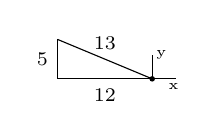
\begin{tikzpicture}[scale=0.1]
\draw (0,0) -- (-12,0) node [pos=0.5, below] {\scriptsize 12};
\draw (-12,0) -- (-12,5) node [pos=0.5, left] {\scriptsize 5};
\draw (0,0) -- (-12,5) node [pos=0.5, above] {\scriptsize 13};

\draw (0,0) -- (3,0) node [pos=0.9, below, yshift=2] {\tiny x};
\draw (0,0) -- (0,3) node [right, xshift=-2] {\tiny y};

\fill (0,0) circle (10pt);
\end{tikzpicture}
\end{adjustbox}

\[ x<-12 \land \sqrt{y^2+z^2} < 5 \Longrightarrow x+r < 1 \Longrightarrow J_0(2\sqrt{x+r}) > 0.22 \]

This implies that the integral of a small block along the negative $x$-axis when $x<-12$ is:

\[ \int_{-1}^{1} \int_{-1}^{1} \int_{x-1}^{x} \left|J_0(2\sqrt{x+r})\right|^2\ dx\ dy\ dz  > 4 \cdot (0.22)^2 \]

Since there are an infinite number of these small blocks, the integral is divergent
and $J_0(2\sqrt{x+r})$ not square integrable.

\end{frame}

\begin{frame}
\begin{exampleblock}{}
\begin{center}
\vskip 20pt
\Huge
Part 2: The solution technique
\vskip 6pt
\ 
\end{center}
\end{exampleblock}
\end{frame}

\begin{frame}
\frametitle{Ansatz 5}

To find the classical solutions to hydrogen, we assumed that the solution was {\it separable}.
This was basically a lucky guess.

\vskip 12pt

Let's make a different assumption (and see if it's lucky, too):

\vskip 12pt

\begin{itemize}
\item The solution satisfies a second-order ODE with rational coefficients

\[ a(v) \frac{d^2 \Psi}{dv^2} + b(v) \frac{d \Psi}{dv} + c(v) \Psi = 0 \]

\item $a(v)$, $b(v)$, $c(v)$ are polynomials in $v$

\item $v$ is a polynomial in $x,y,z,r$

\item $a(v)$, $b(v)$, $c(v)$, and $v$ are all first degree polynomials
\end{itemize}
\end{frame}

\tikzstyle{poly}=[rectangle, draw, thick, fill=white, text width=5em, align=center, rounded corners, minimum height=2em]
\tikzstyle{poly2}=[rectangle, draw, thick, fill=white, align=center, rounded corners, minimum height=2em]
\tikzstyle{ring}=[rectangle, draw=blue, thick, fill=blue!20, text width=5em,align=center, rounded corners, minimum height=2em]
\tikzstyle{element}=[rectangle, draw=orange, thick, fill=orange!20, align=center, rounded corners, minimum height=2em]
\tikzstyle{algebraic}=[rectangle, draw=green, thick, fill=green!20, align=center, rounded corners, minimum height=2em]
\tikzstyle{degree}=[]

\begin{frame}
\frametitle{Ansatz 5}
\begin{center}
  \begin{tikzpicture}[remember picture,out=315,in=225,distance=0.4cm,node distance=40pt]
    \node (Psi) [poly, text width=100pt] {$\framebox(10,10){}\tikzmark{a}\,\Psi'' + \framebox(10,10){}\tikzmark{b}\,\Psi' + \coeff\tikzmark{c}\,\Psi$};
    \node (Qv) [ring, below of=Psi, text width=100pt] {$\mathbf{Q}[v]$};
    \node (v) [poly, right=of Qv] {$v$};
    \draw[degree] (a.west) -- (a.west|-Qv.north) node[right,pos=0.6] {1};
    \draw[degree] (b.west) -- (b.west|-Qv.north) node[right,pos=0.6] {1};
    \draw[degree] (c.west) -- (c.west|-Qv.north) node[right,pos=0.6] {1};
    \node (Psi label) [at=(v.east|-Psi.north), anchor=north east] {\Large$\Psi$};
    \begin{scope}[on background layer]
        \node (Psi block)[fit=(Psi) (Qv) (v), inner sep=10pt, element] {};
    \end{scope}
    \node (base) [ring, node distance=70pt, below=of Psi block.east, anchor=east, text width=250pt] {$\mathbf{Q}[x,y,z,r]/(r^2-x^2-y^2-z^2)$};
    \draw[degree] (v.south) -- (v.south|-base.north) node[right,pos=0.7] {1};
  \end{tikzpicture}
\end{center}

\end{frame}

\begin{frame}
\frametitle{Jet Notation}

\begin{center}
$\frac{\delta^2 \Psi(x,y,z)}{\delta x^2}$ is written as $\Psi_{xx}(x,y,z)$ or just $\Psi_{xx}$
\end{center}
\end{frame}

\begin{frame}
\frametitle{Ansatz 5}

\begin{center}

The Hydrogen PDE:

\[ \frac{1}{2} \Psi_{xx} + \frac{1}{2} \Psi_{yy} + \frac{1}{2} \Psi_{zz} - \frac{1}{r} \Psi = E \Psi \]

\vskip 10pt

Ansatz 5:

\begin{equation*}
\label{ansatz 5a}
v = v_1 x + v_2 y + v_3 z + v_4 r
\end{equation*}

\begin{equation*}
\label{ansatz 5b}
(a_0 + a_1 v) \Psi_{vv} + (b_0 + b_1 v) \Psi_v + (c_0 + c_1 v) \Psi = 0
\end{equation*}

\begin{equation*}
\label{ansatz 5c}
\begin{gathered}
\Psi_x = \Psi_v v_x \qquad
\Psi_y = \Psi_v v_y \qquad
\Psi_z = \Psi_v v_z \\
\Psi_{vx} = \Psi_{vv} v_x \qquad
\Psi_{vy} = \Psi_{vv} v_y \qquad
\Psi_{vz} = \Psi_{vv} v_z \\
\end{gathered}
\end{equation*}

\end{center}

\end{frame}

\begin{frame}
\frametitle{Expansion of $\Psi_{xx}$}

We now substitute ansatz 5 into the hydrogen PDE.

\vskip 12pt

For example, consider the first term in the PDE, $\Psi_{xx}$:

\[ \Psi_{xx} = (\Psi_x)_x = (\Psi_v v_x)_x = \Psi_{vx} v_x + \Psi_v v_{xx} = \Psi_{vv} (v_x)^2 + \Psi_v v_{xx} \]

\[ v_x = \frac{\delta}{\delta x}\left(v_1 x + v_2 y + v_3 z + v_4 r\right) = v_1 + v_4 \frac{x}{r} \]
\[ v_{xx} = v_4 \left(\frac{x^2-r^2}{r^3}\right) \]

\[ \Psi_{vv} = - \frac{ (b_0 + b_1 v) \Psi_v + (c_0 + c_1 v) \Psi } {a_0 + a_1 v} \]

\[ \Psi_{xx} = - \frac{ (b_0 + b_1 v) \Psi_v + (c_0 + c_1 v) \Psi } {a_0 + a_1 v} \left( v_1 + v_4 \frac{x}{r} \right)^2 + v_4 \left(\frac{x^2-r^2}{r^3}\right) \Psi_v \]

\end{frame}

\begin{frame}
\frametitle{The Expanded Numerator}
\tiny
\[
-2 r^4 \Psi E v_0 a_1-r^4 \Psi v_0 v_1^2 c_1-r^4 \Psi v_0 v_2^2 c_1-r^4 \Psi v_0 v_3^2 c_1-r^4 \Psi_v v_0 v_1^2 b_1
-r^4 \Psi_v v_0 v_2^2 b_1-r^4 \Psi_v v_0 v_3^2 b_1
-2 r^3 \Psi x E v_1 a_1
\] \[
-2 r^3 \Psi x v_0^2 v_1 c_1
-r^3 \Psi x v_1^3 c_1-r^3 \Psi x v_1 v_2^2 c_1-r^3 \Psi x v_1 v_3^2 c_1-2 r^3 \Psi y E v_2 a_1
-2 r^3 \Psi y v_0^2 v_2 c_1-r^3 \Psi y v_1^2 v_2 c_1
\] \[
-r^3 \Psi y v_2^3 c_1-r^3 \Psi y v_2 v_3^2 c_1
-2 r^3 \Psi z E v_3 a_1-2 r^3 \Psi z v_0^2 v_3 c_1
-r^3 \Psi z v_1^2 v_3 c_1
-r^3 \Psi z v_2^2 v_3 c_1 -r^3 \Psi z v_3^3 c_1-2 r^3 \Psi E a_0
\] \[
-2 r^3 \Psi v_0 a_1-r^3 \Psi v_1^2 c_0-r^3 \Psi v_2^2 c_0-r^3 \Psi v_3^2 c_0
-2 r^3 \Psi_v x v_0^2 v_1 b_1
-r^3 \Psi_v x v_1^3 b_1-r^3 \Psi_v x v_1 v_2^2 b_1
-r^3 \Psi_v x v_1 v_3^2 b_1
\] \[
-2 r^3 \Psi_v y v_0^2 v_2 b_1-r^3 \Psi_v y v_1^2 v_2 b_1
-r^3 \Psi_v y v_2^3 b_1-r^3 \Psi_v y v_2 v_3^2 b_1-2 r^3 \Psi_v z v_0^2 v_3 b_1-r^3 \Psi_v z v_1^2 v_3 b_1-r^3 \Psi_v z v_2^2 v_3 b_1
\] \[
-r^3 \Psi_v z v_3^3 b_1
-3 r^3 \Psi_v v_0^2 a_1-r^3 \Psi_v v_1^2 b_0-r^3 \Psi_v v_2^2 b_0-r^3 \Psi_v v_3^2 b_0-r^2 \Psi x^2 v_0^3 c_1-2 r^2 \Psi x^2 v_0 v_1^2 c_1
-4 r^2 \Psi x y v_0 v_1 v_2 c_1
\] \[
-4 r^2 \Psi x z v_0 v_1 v_3 c_1
-2 r^2 \Psi x v_0 v_1 c_0-2 r^2 \Psi x v_1 a_1-r^2 \Psi y^2 v_0^3 c_1
-2 r^2 \Psi y^2 v_0 v_2^2 c_1
-4 r^2 \Psi y z v_0 v_2 v_3 c_1
\] \[
-2 r^2 \Psi y v_0 v_2 c_0-2 r^2 \Psi y v_2 a_1-r^2 \Psi z^2 v_0^3 c_1-2 r^2 \Psi z^2 v_0 v_3^2 c_1
-2 r^2 \Psi z v_0 v_3 c_0-2 r^2 \Psi z v_3 a_1-2 r^2 \Psi a_0-r^2 \Psi_v x^2 v_0^3 b_1
\] \[
-2 r^2 \Psi_v x^2 v_0 v_1^2 b_1
-4 r^2 \Psi_v x y v_0 v_1 v_2 b_1
-4 r^2 \Psi_v x z v_0 v_1 v_3 b_1-3 r^2 \Psi_v x v_0 v_1 a_1-2 r^2 \Psi_v x v_0 v_1 b_0
-4 r^2 \Psi_v x z v_0 v_1 v_3 b_1
\] \[
-3 r^2 \Psi_v x v_0 v_1 a_1-2 r^2 \Psi_v x v_0 v_1 b_0
-r^2 \Psi_v y^2 v_0^3 b_1-2 r^2 \Psi_v y^2 v_0 v_2^2 b_1-4 r^2 \Psi_v y z v_0 v_2 v_3 b_1-3 r^2 \Psi_v y v_0 v_2 a_1-2 r^2 \Psi_v y v_0 v_2 b_0
\] \[
-r^2 \Psi_v z^2 v_0^3 b_1-2 r^2 \Psi_v z^2 v_0 v_3^2 b_1-3 r^2 \Psi_v z v_0 v_3 a_1
-2 r^2 \Psi_v z v_0 v_3 b_0
-3 r^2 \Psi_v v_0 a_0
-r \Psi x^3 v_0^2 v_1 c_1-r \Psi x^2 y v_0^2 v_2 c_1
\] \[
-r \Psi x^2 z v_0^2 v_3 c_1
-r \Psi x^2 v_0^2 c_0-r \Psi x y^2 v_0^2 v_1 c_1-r \Psi x z^2 v_0^2 v_1 c_1-r \Psi y^3 v_0^2 v_2 c_1-r \Psi y^2 z v_0^2 v_3 c_1-r \Psi y^2 v_0^2 c_0-r \Psi y z^2 v_0^2 v_2 c_1
\] \[
-r \Psi z^3 v_0^2 v_3 c_1
-r \Psi z^2 v_0^2 c_0
-r \Psi_v x^3 v_0^2 v_1 b_1-r \Psi_v x^2 y v_0^2 v_2 b_1-r \Psi_v x^2 z v_0^2 v_3 b_1+r \Psi_v x^2 v_0^2 a_1-r \Psi_v x^2 v_0^2 b_0
-r \Psi_v x y^2 v_0^2 v_1 b_1
\] \[
-r \Psi_v x z^2 v_0^2 v_1 b_1-r \Psi_v y^3 v_0^2 v_2 b_1-r \Psi_v y^2 z v_0^2 v_3 b_1+r \Psi_v y^2 v_0^2 a_1-r \Psi_v y^2 v_0^2 b_0
-r \Psi_v y z^2 v_0^2 v_2 b_1-r \Psi_v z^3 v_0^2 v_3 b_1
\] \[
+r \Psi_v z^2 v_0^2 a_1-r \Psi_v z^2 v_0^2 b_0
+\Psi_v x^3 v_0 v_1 a_1+\Psi_v x^2 y v_0 v_2 a_1+\Psi_v x^2 z v_0 v_3 a_1+\Psi_v x^2 v_0 a_0+\Psi_v x y^2 v_0 v_1 a_1+\Psi_v x z^2 v_0 v_1 a_1
\] \[
+\Psi_v y^3 v_0 v_2 a_1+\Psi_v y^2 z v_0 v_3 a_1+\Psi_v y^2 v_0 a_0+\Psi_v y z^2 v_0 v_2 a_1+\Psi_v z^3 v_0 v_3 a_1+\Psi_v z^2 v_0 a_0
\]
\end{frame}

\begin{frame}
\frametitle{Collect Like Terms}
Collect like terms in $\Psi$, $\Psi_v$, $x$, $y$, $z$, and $r$.

\[ r\Psi x^3 \left(-2 E a_1 v_1 - 3 c_1 v_0^2 v_1 - c_1 v_1^3 - c_1 v_1 v_2^2 - c_1 v_1 v_3^2\right) - \cdots \]
\end{frame}

\begin{frame}
\frametitle{The System of Equations}
%%\scriptsize
\fontsize{9}{11}\selectfont
\begin{minipage}{.7\linewidth}
\begin{equation*}
\begin{array}{r}
-2 \, c_{1} v_{0}^{3} - 4 \, c_{1} v_{0} v_{1}^{2} - 4 \, c_{1} v_{0} v_{2}^{2} - 2 \, c_{1} v_{0} v_{3}^{2} - 4 \, E a_{1} v_{0} =0\\
-2 \, c_{1} v_{0}^{3} - 4 \, c_{1} v_{0} v_{1}^{2} - 2 \, c_{1} v_{0} v_{2}^{2} - 4 \, c_{1} v_{0} v_{3}^{2} - 4 \, E a_{1} v_{0} =0\\
-2 \, c_{1} v_{0}^{3} - 2 \, c_{1} v_{0} v_{1}^{2} - 4 \, c_{1} v_{0} v_{2}^{2} - 4 \, c_{1} v_{0} v_{3}^{2} - 4 \, E a_{1} v_{0} =0\\
-3 \, b_{1} v_{0}^{2} v_{1} -  \, b_{1} v_{1}^{3} -  \, b_{1} v_{1} v_{2}^{2} -  \, b_{1} v_{1} v_{3}^{2} =0\\
-3 \, b_{1} v_{0}^{2} v_{2} -  \, b_{1} v_{1}^{2} v_{2} -  \, b_{1} v_{2}^{3} -  \, b_{1} v_{2} v_{3}^{2} =0\\
-3 \, b_{1} v_{0}^{2} v_{3} -  \, b_{1} v_{1}^{2} v_{3} -  \, b_{1} v_{2}^{2} v_{3} -  \, b_{1} v_{3}^{3} =0\\
-2 \, b_{1} v_{0}^{3} - 4 \, b_{1} v_{0} v_{1}^{2} - 4 \, b_{1} v_{0} v_{2}^{2} - 2 \, b_{1} v_{0} v_{3}^{2} =0\\
-2 \, b_{1} v_{0}^{3} - 4 \, b_{1} v_{0} v_{1}^{2} - 2 \, b_{1} v_{0} v_{2}^{2} - 4 \, b_{1} v_{0} v_{3}^{2} =0\\
-3 \, c_{1} v_{0}^{2} v_{1} -  \, c_{1} v_{1}^{3} -  \, c_{1} v_{1} v_{2}^{2} -  \, c_{1} v_{1} v_{3}^{2} - 2 \, E a_{1} v_{1} =0\\
-3 \, c_{1} v_{0}^{2} v_{2} -  \, c_{1} v_{1}^{2} v_{2} -  \, c_{1} v_{2}^{3} -  \, c_{1} v_{2} v_{3}^{2} - 2 \, E a_{1} v_{2} =0\\
-3 \, c_{1} v_{0}^{2} v_{3} -  \, c_{1} v_{1}^{2} v_{3} -  \, c_{1} v_{2}^{2} v_{3} -  \, c_{1} v_{3}^{3} - 2 \, E a_{1} v_{3} =0\\
-2 \, b_{1} v_{0}^{3} - 2 \, b_{1} v_{0} v_{1}^{2} - 4 \, b_{1} v_{0} v_{2}^{2} - 4 \, b_{1} v_{0} v_{3}^{2} =0\\
- \, c_{0} v_{0}^{2} -  \, c_{0} v_{1}^{2} -  \, c_{0} v_{2}^{2} -  \, c_{0} v_{3}^{2} - 2 \, E a_{0} - 2 \, a_{1} v_{0} =0\\
- \, c_{1} v_{0}^{3} - 3 \, c_{1} v_{0} v_{1}^{2} -  \, c_{1} v_{0} v_{2}^{2} -  \, c_{1} v_{0} v_{3}^{2} - 2 \, E a_{1} v_{0} =0\\
- \, c_{1} v_{0}^{3} -  \, c_{1} v_{0} v_{1}^{2} - 3 \, c_{1} v_{0} v_{2}^{2} -  \, c_{1} v_{0} v_{3}^{2} - 2 \, E a_{1} v_{0} =0\\
- \, c_{1} v_{0}^{3} -  \, c_{1} v_{0} v_{1}^{2} -  \, c_{1} v_{0} v_{2}^{2} - 3 \, c_{1} v_{0} v_{3}^{2} - 2 \, E a_{1} v_{0} =0\\
-2 \, a_{1} v_{0}^{2} -  \, b_{0} v_{0}^{2} -  \, b_{0} v_{1}^{2} -  \, b_{0} v_{2}^{2} -  \, b_{0} v_{3}^{2} =0\\
- \, b_{1} v_{0}^{3} - 3 \, b_{1} v_{0} v_{1}^{2} -  \, b_{1} v_{0} v_{2}^{2} -  \, b_{1} v_{0} v_{3}^{2} =0\\
- \, b_{1} v_{0}^{3} -  \, b_{1} v_{0} v_{1}^{2} - 3 \, b_{1} v_{0} v_{2}^{2} -  \, b_{1} v_{0} v_{3}^{2} =0\\
- \, b_{1} v_{0}^{3} -  \, b_{1} v_{0} v_{1}^{2} -  \, b_{1} v_{0} v_{2}^{2} - 3 \, b_{1} v_{0} v_{3}^{2} =0
\end{array}
\end{equation*}
\end{minipage}%
\begin{minipage}{.3\linewidth}
\begin{equation*}
\begin{array}{r}
-4 \, b_{1} v_{0} v_{1} v_{2} =0\\
-4 \, b_{1} v_{0} v_{1} v_{3} =0\\
-4 \, b_{1} v_{0} v_{2} v_{3} =0\\
-4 \, c_{1} v_{0} v_{1} v_{2} =0\\
-4 \, c_{1} v_{0} v_{1} v_{3} =0\\
-4 \, c_{1} v_{0} v_{2} v_{3} =0\\
-2 \, c_{0} v_{0} v_{1} - 2 \, a_{1} v_{1} =0\\
-2 \, c_{0} v_{0} v_{2} - 2 \, a_{1} v_{2} =0\\
-2 \, c_{0} v_{0} v_{3} - 2 \, a_{1} v_{3} =0\\
-2 \, a_{1} v_{0} v_{1} - 2 \, b_{0} v_{0} v_{1} =0\\
-2 \, a_{1} v_{0} v_{2} - 2 \, b_{0} v_{0} v_{2} =0\\
-2 \, a_{1} v_{0} v_{3} - 2 \, b_{0} v_{0} v_{3} =0\\
-2 \, a_{0} =0\\
-2 \, a_{0} v_{0} =0\\
\end{array}
\end{equation*}
\end{minipage}
\end{frame}

\begin{frame}
\frametitle{Rings, Ideals and Varieties}
\begin{definition}[commutative algebra]
A {\it commutative ring} is a set of objects closed under two binary operations, addition and multiplication,
that satisfies the following axioms:
\end{definition}

\begin{definition}[commutative algebra]
An {\it ideal} $I$ of a ring $R$ is a subring of $R$ closed under multiplication with elements from $R$:
\[ \forall r \in R, \forall a \in I, ra \in I \]
\end{definition}

\begin{definition}[algebraic geometry]
An {\it algebraic variety} $V$ is the zero locus of some set of polynomials $S$:
\[ V(S) = \{ x \in {\mathbb A}^n | f(x) = 0 \quad\forall f \in S \} \]
\end{definition}
\end{frame}

\begin{frame}
\frametitle{Radical Ideals}
\begin{definition}[commutative algebra]
The {\it radical} of an ideal $I$ of a ring $R$ is:
\[ \sqrt{I} = \{ a \in R \ | \ \exists n \in {\mathbb Z}, a^n \in I \} \]
\end{definition}
\end{frame}

\begin{frame}[fragile]
\frametitle{The Prime Decomposition of the System of Equations}
\begin{verbatim}
sage: I.radical().primary_decomposition()
\end{verbatim}

\begin{subequations}
\label{ideal}
\begin{align}
& \left(n_{1}, n_{0}, m_{1}, m_{0}, d_{1}, d_{0}\right)\label{ideal:5} \\
& \qquad \text{sets all coefficients of the ODE to zero} \nonumber \\
& \left(v_{3}, v_{2}, v_{1}, v_{0}, d_{0}\right)\label{ideal:4}\\
& \qquad \text{sets the variable $v$ to zero} \nonumber \\
& \left(v_{1}^{2} + v_{2}^{2} + v_{3}^{2}, v_{0}, d_{1}, d_{0}\right)\label{ideal:3}\\
& \qquad \text{sets the coefficient of $\Psi_{vv}$ in the ODE to zero} \nonumber \\
& \left(v_{3}, v_{2}, v_{1}, m_{1}, m_{0} - n_{0} v_{0}, 2 d_{1} + n_{0} v_{0}, d_{0}, E n_{0} - n_{1} v_{0}\right)\label{ideal:2}\\
& \qquad \text{the classical solution} \nonumber \\
& \left(v_{0}^{2} - v_{1}^{2} - v_{2}^{2} - v_{3}^{2}, n_{1}, m_{1}, m_{0} - n_{0} v_{0}, d_{1} + n_{0} v_{0}, d_{0}, E\right)\label{ideal:1}\\
& \qquad \text{the new solution} \nonumber
\end{align}
\end{subequations}
\end{frame}

\begin{frame}
\frametitle{Ideal \eqref{ideal:2}}
\[ \left(v_{3}, v_{2}, v_{1}, b_{1}, b_{0} - c_{0} v_{0}, 2 a_{1} + c_{0} v_{0}, a_{0}, E c_{0} - c_{1} v_{0}\right) \]

%% $a_0$ is an ideal generator, so $a_0=0$

We can always multiply our homogenous differential polynomial by a constant without affecting our result, so we can set $a_1=1$.

Likewise, we can multiply our variable $v$ by a constant and that will only change our coefficients by constants,
so set $v_0=1$.
% so we can normalize by setting $v_0=1$.
% and $v_1=v_2=v_3=0$, so we can normalize by setting $v_0=1$.  This simplifies ideal \eqref{ideal:2} to:

\begin{equation*}
\left(v_{3}, v_{2}, v_{1}, v_{0} - 1, c_{0} + 2, b_{1}, b_{0} + 2, a_{1} - 1, a_{0}, 2 E + c_{1}\right)
\end{equation*}

\begin{equation*}
\label{classical eq in ideal}
\begin{gathered}
v=r \\
v \Psi'' + 2 \Psi' + 2(1 + E v) \Psi = 0
\end{gathered}
\end{equation*}

This is the classical radial equation obtained by seperation of variables,
with the orbital quantum number $l=0$,
though it is more commonly written in this form:

\begin{equation*}
\frac{1}{R} \frac{d}{dr}\left[ r^2 \frac{dR}{dr}\right] + 2(Er^2 + r) = 0
\end{equation*}
\end{frame}

\begin{frame}
\frametitle{Ideal \eqref{ideal:1}}
Ideal \eqref{ideal:1} was not expected, and contains our new solution.
$a_0$ is an ideal generator,
so $a_0=0$, and we can set $a_1=1$, by the same logic as above.
Our coordinates are in real space, so our $v_i$ coefficients must be real (why?), so all of their squares must
be positive, and since $v_0^2-v_1^2-v_2^2-v_3^3=0$, $v_0$ must be non-zero.  So we can normalize by setting $v_0=1$.
That simplifies \eqref{ideal:1} to this ideal:

\begin{equation}
\left(v_{1}^{2} + v_{2}^{2} + v_{3}^{2} - 1, v_{0} - 1, c_{1}, c_{0} + 1, b_{1}, b_{0} + 1, a_{1} - 1, a_{0}, E\right)
\end{equation}

This ideal corresponds to the following system of equations:

\begin{equation}
\begin{gathered}
E = 0 \\
a_0 = 0 \qquad
a_1 = 1 \\
b_0 = -1 \qquad
b_1 = 0 \\
c_0 = -1 \qquad
n_1 = 0 \\
v_0 = 1 \qquad
v_1^2 + v_2^2 + v_3^2 = 1
\end{gathered}
\end{equation}

\end{frame}

\begin{frame}
\frametitle{Ideal \eqref{ideal:1} (cont)}

Substituting these values back into our ansatz, we conclude that $\Psi(v)$
is a solution of \eqref{schrodinger} under these conditions:

\begin{equation}
\label{related solution}
\begin{gathered}
v \frac{\delta^2\Psi}{\delta v^2} + \frac{\delta\Psi}{\delta v} + \Psi = 0 \\
v = v_1 x+ v_2 y+ v_3 z+r \\
v_1^2 + v_2^2 + v_3^2 = 1
\end{gathered}
\end{equation}

The expression $v_1 x + v_2 y + v_3 z$ is easily identified as a dot product between
the coordinate $(x,y,z)$ and the unit vector $(v_1, v_2, v_3)$ (remembering
that $v_1^2 + v_2^2 + v_3^2 = 1$).  The direction of this vector is arbitrary,
so we can orient the $x$-axis in this direction and set $(v_1, v_2, v_3) = (1,0,0)$
without loss of generality.

We now have to solve a second order ODE:

\begin{equation}
v \Psi''(v) + \Psi'(v) + \Psi(v) = 0
\end{equation}

\end{frame}

\begin{frame}
\frametitle{Ideal \eqref{ideal:1} (cont)}

Wolfram Mathematica can now
analyze this equation and determine that it can be solved with Bessel functions:

\includegraphics[page=1, clip, trim=1in 9in 1in 0.5in, width=\textwidth]{find Bessel solution.pdf}

{\tt BesselY} is a Bessel function of the second kind.  It has a singularity at $x=0$ and is also not square integrable.

\vskip 12pt

Plugging in $v=x+r$, we obtain:

\[ \psi(x,y,z) = J_0(2\sqrt{x+r}) \]
\end{frame}

\begin{frame}
\frametitle{Key Takeaway Points}
\begin{itemize}
\item Separation of variables only finds separable solutions\\ (there may be others)
\item It's not enough to solve the Schr\"odinger differential equation\\The wavefunction also has to be square integrable
\item Ideals are the principal algebraic tool for analyzing systems of polynomial equations
\item Forming the radical of an ideal introduces the additional axiom that there are no zero divisors
\item The preferred approach to analyzing a difficult ideal
is to construct a primary decomposition of its radical
\end{itemize}
\end{frame}

\begin{frame}
\begin{exampleblock}{}
\begin{center}
\vskip 20pt
\Huge
Part 3: Moving the Research Project Forward
\vskip 6pt
\ 
\end{center}
\end{exampleblock}
\end{frame}

\begin{frame}
\frametitle{Methods of Solving Systems of Polynomial Equations}
\begin{itemize}
\item Primary Decomposition with Gr\"obner Bases
\item Numerical Optimization
\item Homotopy Continuation
\end{itemize}
\end{frame}

\begin{frame}
\frametitle{Numerical Optimization}
\begin{itemize}
\item Use numerical root-finding techniques (gradient descent, Levenburg-Marquardt, {\tt scipy}) to find an approximate zero
\item We get a {\it witness point}: an approximate solution good enough to recover the exact solution ({\it exactness recovery})
\item Ex: 1.0000057 is approximately 1
\item This works well for finding a single prime component
\item The problem is how to remove a prime component so you can find all the prime components
\end{itemize}
\end{frame}

\begin{frame}
\frametitle{The Euclidean Distance Function}
\end{frame}

\begin{frame}
\frametitle{Use of Large Language Models in Software Development}
\end{frame}

\end{document}
